\documentclass[letterpaper,11pt]{article}
\usepackage{graphicx}
\usepackage{listings}
\usepackage[super]{nth}
\usepackage[hyphens]{url}
\usepackage{amsmath}
\usepackage[makeroom]{cancel}
\usepackage[table]{xcolor}
\usepackage{comment}
\usepackage[space]{grffile}

\lstset{
	basicstyle=\footnotesize,
	breaklines=true,
}

\begin{document}

\begin{titlepage}

\begin{center}

\Huge{Assignment 5}

\Large{CS 595:  Introduction to Web Science}

\Large{Fall 2013}

\Large{Shawn M. Jones}

\Large Finished on \today

\end{center}

\end{titlepage}

\newpage
\section*{1}

\subsection*{Question}

\begin{verbatim}
1.  Determine if the friendship paradox holds for your Facebook account.  
Create a graph of the number of friends (y-axis) and the friends sorted
by number of friends (x-axis).  (The friends don't need to be labeled 
on the x-axis.)  Do include yourself in the graph and label yourself
accordingly.

Compute the mean, standard deviation, and median of the number of friends
that your friends have.

You can download your network in an XML file by using the NameGenWeb
Facebook app: 

https://apps.facebook.com/namegenweb/ 

You will need to give this app permission to access your Facebook
data. Make sure you select "Friend Count" as an Extended Attribute.
When you download the data, download it in the GraphML format.

If you do not have a Facebook account, email me and I will send you 
my GraphML file.
\end{verbatim}

\newpage
\subsection*{Answer}

Downloading the graphl file from the NameGenWeb gave me nothing when I anonymized it, so I had to work with the non-anonymized data.  The Python script \verb+processFBGraph.py+ used to process it is shown in Listing \ref{lst:q1codepy}.  It turns the data into a comma-separated stream that can be output to a file as shown below.

\begin{lstlisting}[frame=single]
./processFBGraph.py not-anonymized-fb-data.graphml > fb-frienddata.csv
\end{lstlisting}

Processing the data was yet another adventure, the script shown in Listing \ref{lst:q1codeR}, its statistics shown in Table \ref{tab:q1stats}, and the graph shown in Figure \ref{fig:q1barplot}.

The R script runs like so:
\begin{lstlisting}[frame=single]
bash $ --> ./processFBGraphOutput.R fb-frienddata.csv q1-barplot.png 154 'ME!!!'
Mean:  302.555555555556
Median:  225.5
Std Dev:  236.389147508571
null device 
          1 
\end{lstlisting}

Seeing as I am the only person with 154 friends on my circle, I was able to color the single bar red using the code on lines 34 and 35 in Listing \ref{lst:q1codeR}.

Figure \ref{fig:q1barplot} shows that I am more popular than about 25\% of my friends, but my friends do have more friends than I do.  Referencing Table \ref{tab:q1stats}, I have fewer friends than the median.

\begin{table}
\begin{tabular}{ l l }
\hline
\textbf{Mean} & 302.555555555556 \\
\textbf{Median} & 225.5 \\
\textbf{Std Dev} & 236.389147508571 \\
\hline
\end{tabular}
\caption{Statistics on the count of my Facebook Friends' Friends, values straight from R}
\label{tab:q1stats}
\end{table}

\clearpage
\begin{figure}[h]
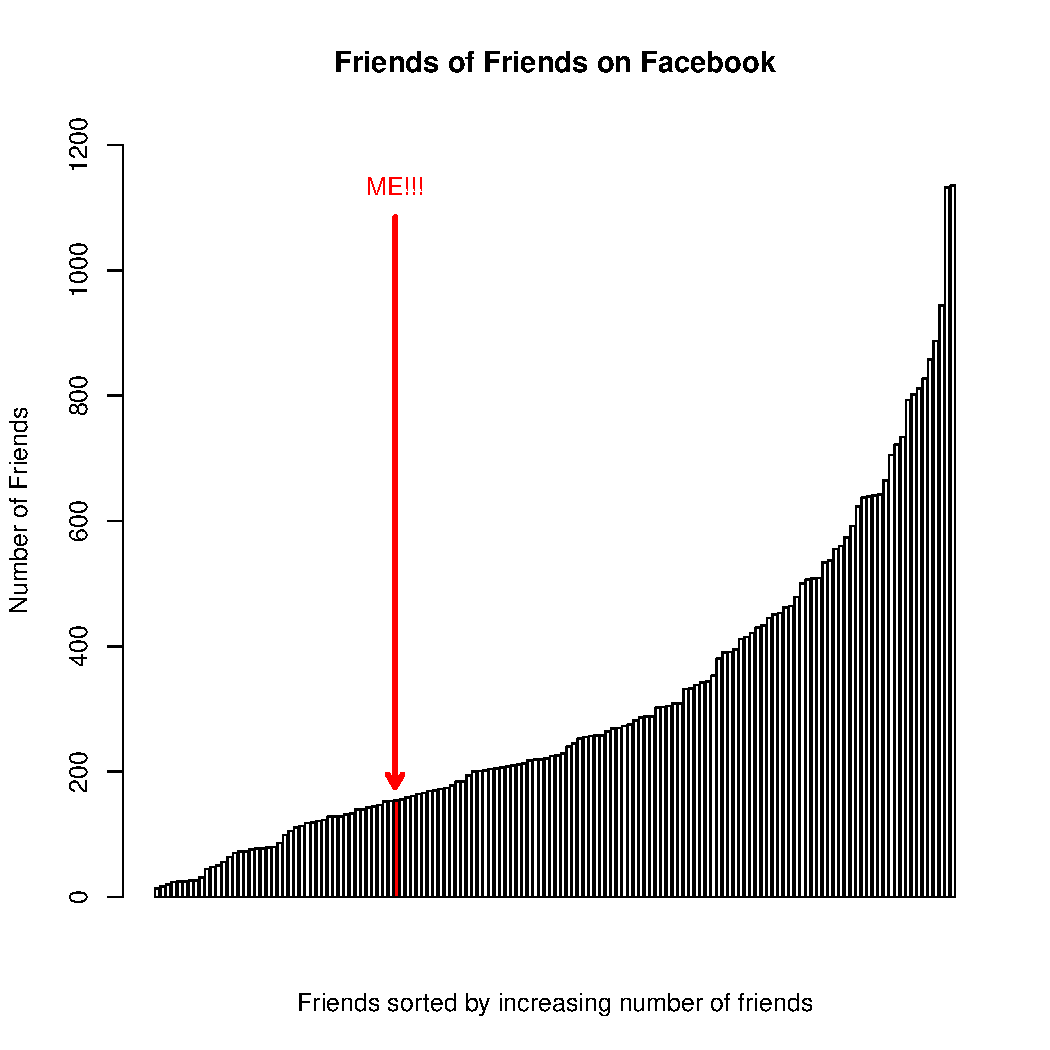
\includegraphics[scale=0.7]{q1/q1-barplot.pdf}
\caption{Bar plot showing the count of my Facebook Friends' Friends}
\label{fig:q1barplot}
\end{figure}

\newpage
\lstinputlisting[language=Python,frame=single,caption={Python program for processing GraphML file from NameGenWeb Facebook App},label=lst:q1codepy,captionpos=b,numbers=left,showspaces=false,showstringspaces=false,basicstyle=\footnotesize]{q1/processFBGraph.py}

\newpage
\lstinputlisting[language=R,frame=single,caption={R program for bar plot shown in Figure \ref{fig:q1barplot}},label=lst:q1codeR,captionpos=b,numbers=left,showspaces=false,showstringspaces=false,basicstyle=\footnotesize]{q1/processFBGraphOutput.R}


\newpage
\section*{2}

\subsection*{Question}

\begin{verbatim}
2.  Determine if the friendship paradox holds for your Twitter account.
Since Twitter is a directed graph, use "followers" as value you measure
(i.e., "do your followers have more followers than you?").

Generate the same graph as in question #1, and calcuate the same 
mean, standard deviation, and median values.

For the Twitter 1.1 API to help gather this data, see:

https://dev.twitter.com/docs/api/1.1/get/followers/list

If you do not have followers on Twitter (or don't have more than 20),
then use my twitter account "phonedude_mln".
\end{verbatim}

\newpage
\subsection*{Answer}

Because I use Twitter as more of a \emph{content consumption} service, I have very few followers, so few that I lack sufficient sample size to actually answer ``do your followers have more followers than you?''.  Fortunately, I have \verb+phonedude_mln+ that I can test with.

The first script, shown in Listing \ref{lst:q2codepy}, queries the Twitter API for information on the followers of \verb+phonedude_mln+ using the function on lines $84$-$98$ and then prints it using the function on lines $100$ - $124$.

This script is run like below, to produce a CSV file.
\begin{lstlisting}[frame=single]
./countTwitterFollowers.py 2 phonedude_mln > phonedude_mln.csv
\end{lstlisting}

From the output, I can see that \verb+phonedude_mln+ has $201$ followers.  The R script shown in Listing \ref{lst:q2codeR} creates a similar bar plot to that shown in answer one and produces the statistics shown in \ref{tab:q2stats}.

\begin{lstlisting}[frame=single]
bash $ --> ./processTwitterFollowerOutput.R phonedude_mln.csv q2-barplot.pdf 201 "phonedude_mln"
Mean:  520.846534653465
Median:  199
Std Dev:  1264.79341369106
null device 
          1 
\end{lstlisting}

It turns out that \verb+phonedude_mln+ is doing better on Twitter than I am doing on Facebook.  He has more followers than the median of $199$, but his followers still have more followers than he does.

\begin{table}
\begin{tabular}{ l l }
\hline
\textbf{Mean} & 520.846534653465 \\
\textbf{Median} & 199 \\
\textbf{Std Dev} & 1264.79341369106 \\
\hline
\end{tabular}
\caption{Statistics on the count of phonedude\_mln's Twitter followers' followers, values straight from R}
\label{tab:q2stats}
\end{table}

\clearpage
\begin{figure}[h]
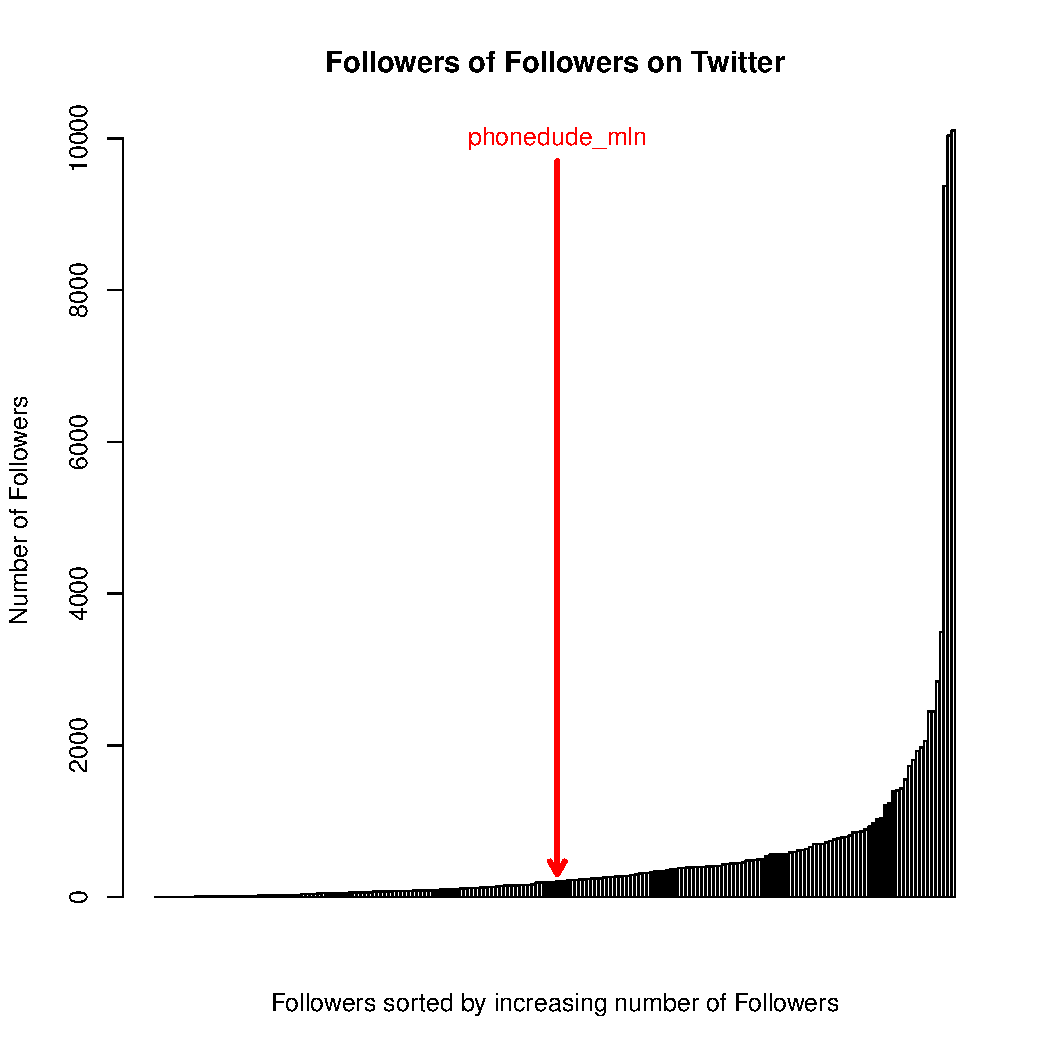
\includegraphics[scale=0.7]{q2/q2-barplot.pdf}
\caption{Bar plot showing the count of phonedude\_mln's Twitter followers' followers}
\label{fig:q2barplot}
\end{figure}


\newpage
\lstinputlisting[language=Python,frame=single,caption={Python program for acquiring Twitter followers for phonedude\_mln},label=lst:q2codepy,captionpos=b,numbers=left,showspaces=false,showstringspaces=false,basicstyle=\footnotesize]{q2/countTwitterFollowers.py}

\newpage
\lstinputlisting[language=R,frame=single,caption={R program for bar plot shown in Figure \ref{fig:q2barplot}},label=lst:q2codeR,captionpos=b,numbers=left,showspaces=false,showstringspaces=false,basicstyle=\footnotesize]{q2/processTwitterFollowerOutput.R}



\newpage
\section*{3}

\subsection*{Question}

\begin{verbatim}
Extra credit, 2 points:

3.  Repeat question #1, but with your LinkedIn profile.
\end{verbatim}

\newpage
\subsection*{Answer}

Not attempted.

\newpage
\section*{4}

\subsection*{Question}

\begin{verbatim}
Extra credit, 1 point:

4.  Repeat question #2, but change "followers" to "following"?  In
other words, are the people I am following following more people?
\end{verbatim}

\newpage
\subsection*{Answer}

Not attempted.


\clearpage
\bibliographystyle{acm}
\bibliography{references}

\end{document}